%!TEX program = xelatex
\documentclass[aspectratio=169,10pt]{ctexbeamer}
\usepackage[bluetheme]{ustcbeamer}
% !TeX root = ./main.tex

% 自适应16:9的宽高比设置
\makeatletter
\@ifclasswith{ctexbeamer}{aspectratio=169}{
		\def\backxscale{4/3}\def\backyscale{1}\def\ustcshift{30}
	}{
		\def\backxscale{1.068}\def\backyscale{1.068}\def\ustcshift{0}
	}
\makeatother

\newcommand{\maketitleframe}{
	%取消footline,sidebar
	\setbeamertemplate{footline}[footlineoff]
	%%设置本命令以后的背景如下
	\usebackgroundtemplate{%
			% !TeX root = ./main.tex
\begin{tikzpicture}[y=1pt, x=1pt, yscale=0.474*\backyscale, xscale=0.474*\backxscale, inner sep=0pt, outer sep=0pt]
    % \begin{scope}[cm={{1,0.0,0.0,-1,(0,0)}}]
      \path[fill=themecolor1,even odd rule] (720.4059,0.3515) -- (720.4059,71.1507) --
        (0.3436,71.1507) -- (0.3436,0.3515) -- cycle;
    
    
    
      \path[fill=themecolor2,even odd rule] (0.3436,76.0927) -- (720.4059,76.0927) --
        (720.4059,79.3043) -- (0.3436,79.3043) -- cycle;
    
    
    
      \path[left color=themecolor!80, right color=themecolor,even odd rule] (720.4059,392.4714) -- (0.3436,392.4714) --
        (0.3436,112.2780) -- (720.4059,112.2780) -- cycle;
    
    
    
          \path[even odd rule] (720.4059,392.4714) -- (0.3436,392.4714) --
            (0.3436,112.2780) -- (720.4059,112.2780) -- cycle;
    
    
    
      \path[fill=themecolor1,even odd rule] (0.3436,540.3980) -- (720.4059,540.3980) --
        (720.4059,433.5987) -- (0.3436,433.5987) -- cycle;
    
    
    
      \path[fill=themecolor,even odd rule] (84.0129,392.4714) -- (64.1007,392.4714) ..
        controls (139.6636,296.8146) and (237.7485,213.1007) .. (369.3679,152.9909) ..
        controls (258.0055,213.1787) and (160.4523,292.5573) .. (84.0129,392.4714) --
        cycle(0.3436,210.9419) -- (0.3436,112.2780) -- (205.1827,112.2780) .. controls
        (135.2103,142.0132) and (67.0535,175.1304) .. (0.3436,210.9419) --
        cycle(0.3436,318.0849) -- (0.3436,261.2429) .. controls (87.4868,197.7318) and
        (173.6552,147.4217) .. (257.6874,112.2780) -- (329.6364,112.2780) .. controls
        (208.4627,165.2559) and (97.0387,225.2988) .. (0.3436,318.0849) --
        cycle(23.7974,392.4714) -- (0.3436,392.4714) -- (0.3436,375.5798) .. controls
        (103.8628,248.3597) and (243.0859,163.2623) .. (385.7678,112.2780) --
        (411.7601,112.2780) .. controls (266.1313,174.0682) and (125.2848,246.4444) ..
        (23.7974,392.4714);
    
    
    
      \path[fill=themecolor2,even odd rule] (0.3436,428.6568) -- (720.4059,428.6568) --
        (720.4059,425.4452) -- (0.3436,425.4452) -- cycle;

      \node at(185-\ustcshift,488){\textcolor{themecolor}{
\includegraphics[scale=1]{./theme/ustc_logo_side.pdf}}};
    % \end{scope}
\end{tikzpicture}
	}%
	%封面页
	\begin{frame}%
		\maketitle%
	\end{frame}%
	%设置本命令以后的背景如下
	\usebackgroundtemplate{%
			% !TeX root = ./main.tex
\begin{tikzpicture}[y=1pt, x=1pt, yscale=0.474*\backyscale, xscale=0.474*\backxscale, inner sep=0pt, outer sep=0pt]
% \begin{scope}[cm={{1,0.0,0.0,-1,(0,0)}}]
    \path[left color=themecolor!80,right color=themecolor,even odd rule] (720.4059,540.3980) -- (0.3436,540.3980) --
      (0.3436,478.8258) -- (720.4059,478.8258) -- cycle;



        \path[even odd rule] (720.4059,540.3980) -- (0.3436,540.3980) --
          (0.3436,478.8258) -- (720.4059,478.8258) -- cycle;



    \path[fill=themecolor,even odd rule] (84.0129,540.3980) -- (64.1007,540.3980) ..
      controls (139.6636,519.3777) and (237.7485,500.9814) .. (369.3679,487.7725) ..
      controls (258.0055,500.9987) and (160.4523,518.4420) .. (84.0129,540.3980) --
      cycle(0.3436,500.5071) -- (0.3436,478.8258) -- (205.1827,478.8258) .. controls
      (135.2103,485.3599) and (67.0535,492.6376) .. (0.3436,500.5071) --
      cycle(0.3436,524.0517) -- (0.3436,511.5606) .. controls (87.4868,497.6042) and
      (173.6552,486.5485) .. (257.6874,478.8258) -- (329.6364,478.8258) .. controls
      (208.4627,490.4677) and (97.0387,503.6621) .. (0.3436,524.0517) --
      cycle(23.7974,540.3980) -- (0.3436,540.3980) -- (0.3436,536.6860) .. controls
      (103.8628,508.7296) and (243.0859,490.0294) .. (385.7678,478.8258) --
      (411.7601,478.8258) .. controls (266.1313,492.4040) and (125.2848,508.3087) ..
      (23.7974,540.3980);

  \path[fill=themecolor2,even odd rule] (720.4059,475.6141) -- (0.3436,475.6141) --
    (0.3436,478.8258) -- (720.4059,478.8258) -- cycle;



  \path[fill=themecolor,even odd rule] (0.3436,0.3515) -- (720.4059,0.3515) --
    (720.4059,28.5100) -- (0.3436,28.5100) -- cycle;



  \path[fill=themecolor2,even odd rule] (720.4059,28.5100) -- (0.3436,28.5100) --
    (0.3436,31.7217) -- (720.4059,31.7217) -- cycle;

  \node at(580+\ustcshift,509){\textcolor{white}{
\includegraphics[scale=0.8]{./theme/ustc_logo_side.pdf}}};



% \end{scope}

\end{tikzpicture}
	}%
}%
%
\usepackage{booktabs,graphicx,amsmath,array,tabularx}
\usepackage{hyperref}
\setbeamertemplate{navigation symbols}{}

\definecolor{positive}{HTML}{0173B2}
\definecolor{negative}{HTML}{9C5700}
\definecolor{emphasis}{HTML}{006E53}
\definecolor{neutral}{HTML}{555555}
\newcommand{\pos}[1]{\textcolor{positive}{#1}}
\newcommand{\con}[1]{\textcolor{negative}{#1}}
\newcommand{\HL}[1]{\textcolor{emphasis}{#1}}
\newcommand{\paperref}[1]{\par\vfill{\raggedleft\scriptsize\textcolor{neutral}{#1}\par}}
\newcommand{\pp}{\,\text{个百分点}}

\title[YOLO-GN+BIFPN]{基于 YOLOv11 的火焰与烟雾检测}
\subtitle{Ghost 模块、BiFPN 与图像增强：论文精读和复现结果}
\author[组会汇报]{组会论文汇报}
\institute[USTC Beamer]{\emph{Engineering Applications of Artificial Intelligence}, 2026}
\date{2026 年 10 月}

\begin{document}
\maketitleframe
\setbeamertemplate{footline}[footlineon]

\begin{frame}{期刊与论文信息}
  \begin{columns}[T,onlytextwidth]
    \begin{column}{.58\textwidth}
      {\Large\bfseries Engineering Applications of Artificial Intelligence}\par\medskip
      Elsevier 工程人工智能应用方向期刊\par\smallskip
      \textbf{中国科学院期刊分区（2025 升级版）}\par
      大类：计算机科学 1 区、工程技术 1 区；相关小类为 2 区。\par\medskip
      \textbf{本文状态：非开放获取}\par
      ScienceDirect 页面显示需机构访问或购买 PDF。\par\medskip
      \textbf{论文：}Improving fire and smoke detection with ghost convolutions, Bidirectional Feature Pyramid Networks, and image enhancement\par
      \small Dewi et al.，Vol. 178, Part 2, Article 115116，2026-08-15\par
      \small DOI: \url{https://doi.org/10.1016/j.engappai.2026.115116}
    \end{column}
    \begin{column}{.38\textwidth}
      \vspace{.2cm}
      {\Large\bfseries 这篇论文的定位}\par\medskip
      \begin{itemize}
        \item 任务：RGB 图像中的 Fire + Smoke 双类别检测
        \item 基础模型：YOLOv11s
        \item 重点：低对比烟雾、多尺度特征和计算效率
        \item 论文报告：CLAHE+CS 与改进模型组合达到 89.50\% mAP
      \end{itemize}
      \vspace{.15cm}
      {\footnotesize 分区信息为 2025 版期刊级分区，引用时以学校图书馆数据库为准。}
    \end{column}
  \end{columns}
  \paperref{ScienceDirect 论文页；科研通《中科院期刊分区》2025 升级版，查询于 2026-10-24}
\end{frame}

\begin{frame}{背景：监控画面中，烟雾可能先于清楚的火焰出现}
  \begin{columns}[T,onlytextwidth]
    \begin{column}{.48\textwidth}
      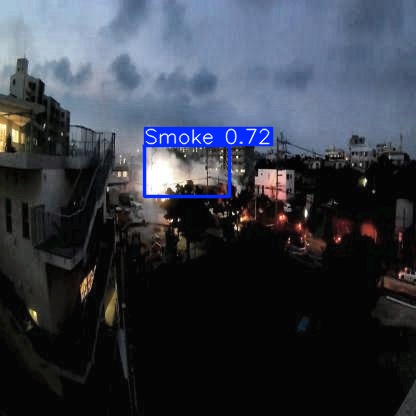
\includegraphics[width=\linewidth]{assets/predictions/test_smoke.jpg}
      \par\centering{\scriptsize 测试集烟雾样例：模型预测框}
    \end{column}
    \begin{column}{.48\textwidth}
      \large
      \begin{itemize}
        \item 野火监测要尽早发现火情；卫星监测覆盖和响应速度有局限。
        \item 远处火焰可能很小，烟羽则范围大、边界淡，两个目标的外观差异明显。
        \item RGB 相机便于连续观察，但云雾、天空和光照变化会让淡烟难辨。
      \end{itemize}
      \vspace{.25cm}
      \textbf{论文关注：}让模型在复杂、低对比画面中更稳地识别火焰与烟雾。
    \end{column}
  \end{columns}
  \paperref{Dewi et al.（2026），Abstract、§1；测试集样例由本次 best.pt 推理}
\end{frame}

\begin{frame}{检测难点：看得见、分得清、算得动}
  \renewcommand{\arraystretch}{1.5}
  \begin{tabularx}{\linewidth}{p{2.15cm}X p{4.05cm}}
    \toprule
    难点 & 画面里是什么情况 & 论文对应的处理\\
    \midrule
    淡烟低对比 & 烟雾与天空、云雾的颜色和纹理接近，容易漏掉或误检 & CLAHE + Contrast Stretching 拉开局部亮度差\\
    尺度变化 & 烟羽可很小，火焰也可能只占少量像素 & P4 层的 BiFPN 融合多层特征\\
    计算开销 & 多分支、多尺度结构会增加推理成本 & Ghost 模块以较少计算生成特征\\
    \bottomrule
  \end{tabularx}
  \vspace{.35cm}
  \begin{alertblock}{需要分清}
    这些模块是针对问题的设计思路；论文结果说明组合模型有效，不等于每类困难都已被单独证明解决。
  \end{alertblock}
  \paperref{Dewi et al.（2026），Abstract、Highlights、§2}
\end{frame}

\begin{frame}{论文方案：图像先增强，检测网络再融合特征}
  \begin{columns}[T,onlytextwidth]
    \begin{column}{.55\textwidth}
      \large
      \begin{enumerate}
        \item 输入 RGB 图像
        \item 用 CLAHE 与 Contrast Stretching 增强对比度
        \item YOLOv11s 主干和颈部加入 Ghost 模块
        \item 在 P4 特征层接入 BiFPN，融合不同尺度的信息
        \item 输出 Fire / Smoke 的框、类别与置信度
      \end{enumerate}
    \end{column}
    \begin{column}{.41\textwidth}
      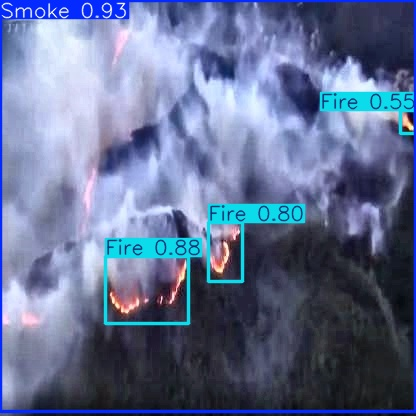
\includegraphics[width=\linewidth,height=.48\textheight,keepaspectratio]{assets/predictions/test_smoke_fire.jpg}
      \par\centering{\scriptsize 测试集火焰与烟雾同框样例}
      \vspace{.1cm}
      \small 输出 Fire / Smoke 的框、类别和置信度。
    \end{column}
  \end{columns}
  \paperref{Dewi et al.（2026），Highlights、§2；示例为本次模型测试集输出}
\end{frame}

\begin{frame}{Ghost 模块：少做重复计算，保留有用特征}
  \begin{columns}[T,onlytextwidth]
    \begin{column}{.52\textwidth}
      \textbf{普通卷积}\par\smallskip
      对输入做卷积，直接计算多张输出特征图，成本较高。\par\medskip
      \textbf{Ghost 思路}\par\smallskip
      先算一部分主要特征，再用较轻的变换补出相关特征，减少重复的完整卷积。\par\medskip
      \textbf{论文放置位置}\par\smallskip
      Backbone 与 Neck 中均引入 Ghost 模块，构成 YOLOv11s-GN。
    \end{column}
    \begin{column}{.43\textwidth}
      \begin{block}{用人话理解}
        有些特征图彼此很像。Ghost 先算代表性的那部分，再用便宜的操作补齐，目标是省计算量。
      \end{block}
      \vspace{.25cm}
      \textbf{它不负责什么？}\par\smallskip
      Ghost 不直接判断是不是烟；它改变的是网络提取特征的计算方式。
    \end{column}
  \end{columns}
  \paperref{Dewi et al.（2026），Highlights、§2.1；GhostNet 原理见论文参考文献}
\end{frame}

\begin{frame}{BiFPN：把不同分辨率的线索合起来}
  \begin{columns}[T,onlytextwidth]
    \begin{column}{.49\textwidth}
      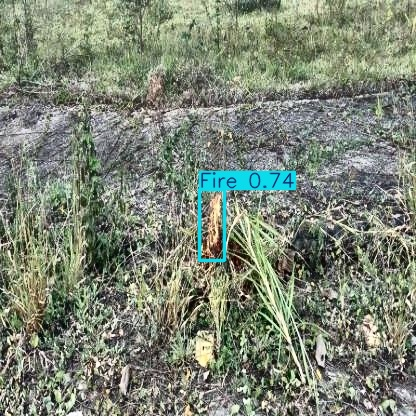
\includegraphics[width=\linewidth,height=.48\textheight,keepaspectratio]{assets/predictions/test_fire.jpg}
      \par\centering{\scriptsize 测试集小目标火焰样例}
    \end{column}
    \begin{column}{.47\textwidth}
      \normalsize
      \begin{itemize}
        \item P3 保留较细的空间位置，适合看小目标。
        \item P4、P5 网格更粗，能带入更大范围的语义信息。
        \item BiFPN 让特征沿自上而下和自下而上的路径传递，再进行加权融合。
        \item 论文把 BiFPN 放在 P4 阶段，目标是兼顾不同尺度的火与烟。
      \end{itemize}
      \vspace{.2cm}
      \textbf{通俗理解：}既看局部细节，也参考周围和更大范围的场景。
    \end{column}
  \end{columns}
  \paperref{Dewi et al.（2026），§2.2；结构连接见本项目模型 YAML}
\end{frame}

\begin{frame}{CLAHE + CS：增强暗淡、接近背景的线索}
  \begin{columns}[T,onlytextwidth]
    \begin{column}{.48\textwidth}
      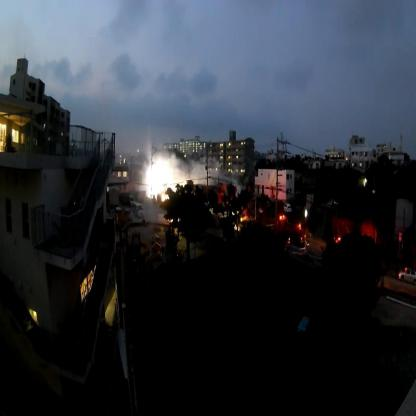
\includegraphics[width=\linewidth,height=.48\textheight,keepaspectratio]{assets/preprocess/source.jpg}
      \par\centering{\scriptsize 原始测试图像}
    \end{column}
    \begin{column}{.48\textwidth}
      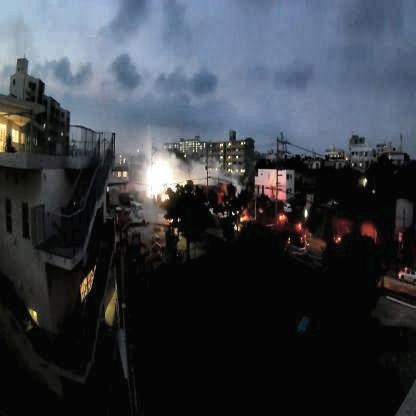
\includegraphics[width=\linewidth,height=.48\textheight,keepaspectratio]{assets/preprocess/clahe_cs.jpg}
      \par\centering{\scriptsize 本次采用 CLAHE + CS 后的输入}
    \end{column}
  \end{columns}
  \vspace{.12cm}
  \small
  CLAHE 提高局部对比度，CS 拉开强度范围。论文还比较 HE、DGC 等方法，报告 CLAHE+CS 组合效果最好（89.50\% mAP）。\par
  \footnotesize 右图为本项目实现；公开信息不足以核实作者的全部增强参数。
  \paperref{Dewi et al.（2026），§2.3；右图为本项目预处理结果}
\end{frame}

\begin{frame}{数据集：Fire and Smoke Dataset}
  \begin{columns}[T,onlytextwidth]
    \begin{column}{.5\textwidth}
      \renewcommand{\arraystretch}{1.45}
      \begin{tabular}{lr}
        \toprule
        固定划分 & 图像数\\
        \midrule
        Train & 8,494\\
        Validation & 2,114\\
        Test & 1,059\\
        \midrule
        合计 & 11,667\\
        \bottomrule
      \end{tabular}
      \vspace{.3cm}
      \begin{itemize}
        \item RGB 图像；类别是 Smoke 和 Fire。
        \item 沿用数据集给出的 train / valid / test 划分。
        \item 本次只用 train 训练、valid 观察过程，最后在 test 报告结果。
      \end{itemize}
    \end{column}
    \begin{column}{.46\textwidth}
      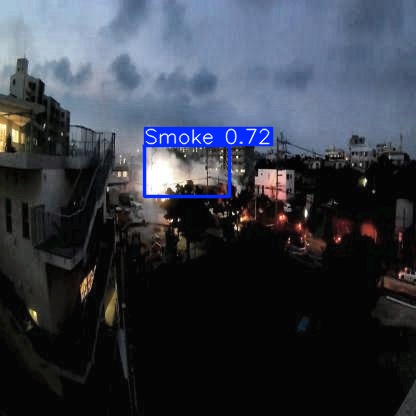
\includegraphics[width=\linewidth,height=.48\textheight,keepaspectratio]{assets/predictions/test_smoke.jpg}
      \par\centering{\scriptsize 测试集中的烟雾场景}
      \vspace{.12cm}
      \small 一张图可有多个框，也可能同时包含火和烟。
    \end{column}
  \end{columns}
  \paperref{Dewi et al.（2026），§3.1；数据源：vinchole/zzzccc}
\end{frame}

\begin{frame}{复现设置：按你的要求从随机初始化训练}
  \small
  \renewcommand{\arraystretch}{1.22}
  \begin{tabularx}{\linewidth}{p{2.45cm}X p{2.9cm}}
    \toprule
    项目 & 本次设置 & 备注\\
    \midrule
    初始化 & \texttt{pretrained=False} & 没有加载预训练权重\\
    输入尺寸 & $640\times640$ & 与 YOLO 常用设置一致\\
    训练轮数 / batch & 300 / 40 & RTX 5090，GPU 3\\
    优化器 & SGD，初始学习率 0.01 & seed 42\\
    训练数据 & CLAHE + CS 版本 & 保留官方固定划分\\
    完成时间 & 约 3 小时 29 分钟 & 单次训练\\
    \bottomrule
  \end{tabularx}
  \vspace{.18cm}
  \begin{alertblock}{复现差异}
    本次从零初始化；作者 Notebook 使用预训练权重，且公开实现中部分结构细节无法独立核验。因此结果是独立复现参考。
  \end{alertblock}
  \paperref{训练参数见本项目脚本；差异依据作者仓库 README 与 Notebook}
\end{frame}

\begin{frame}{配置文件各管一件事}
  \begin{columns}[T,onlytextwidth]
    \begin{column}{.31\textwidth}
      \textbf{模型 YAML}\par\medskip
      {\ttfamily\small yolo11s\_gn\_bifpn.yaml}\par\medskip
      说明网络每一层接谁、使用什么模块、检测头读取哪些尺度。
    \end{column}
    \begin{column}{.31\textwidth}
      \textbf{数据 YAML}\par\medskip
      {\ttfamily\small data\_clahe\_cs.yaml}\par\medskip
      指向 train / valid / test 文件夹，并写明类别顺序：Smoke、Fire。
    \end{column}
    \begin{column}{.31\textwidth}
      \textbf{训练脚本}\par\medskip
      {\ttfamily\small train.py}\par\medskip
      指定 batch、轮数、优化器、GPU，以及 \texttt{pretrained=False}。
    \end{column}
  \end{columns}
  \vspace{.4cm}
  \begin{block}{一句话}
    模型 YAML 决定“网络长什么样”，数据 YAML 决定“读哪些图和标签”，训练脚本决定“怎么学”。
  \end{block}
  \paperref{本项目配置文件；模型模块实现见 \texttt{models/ghost\_bifpn.py}}
\end{frame}

\begin{frame}{训练曲线：loss 持续下降，验证 mAP 稳步上升}
  \centering
  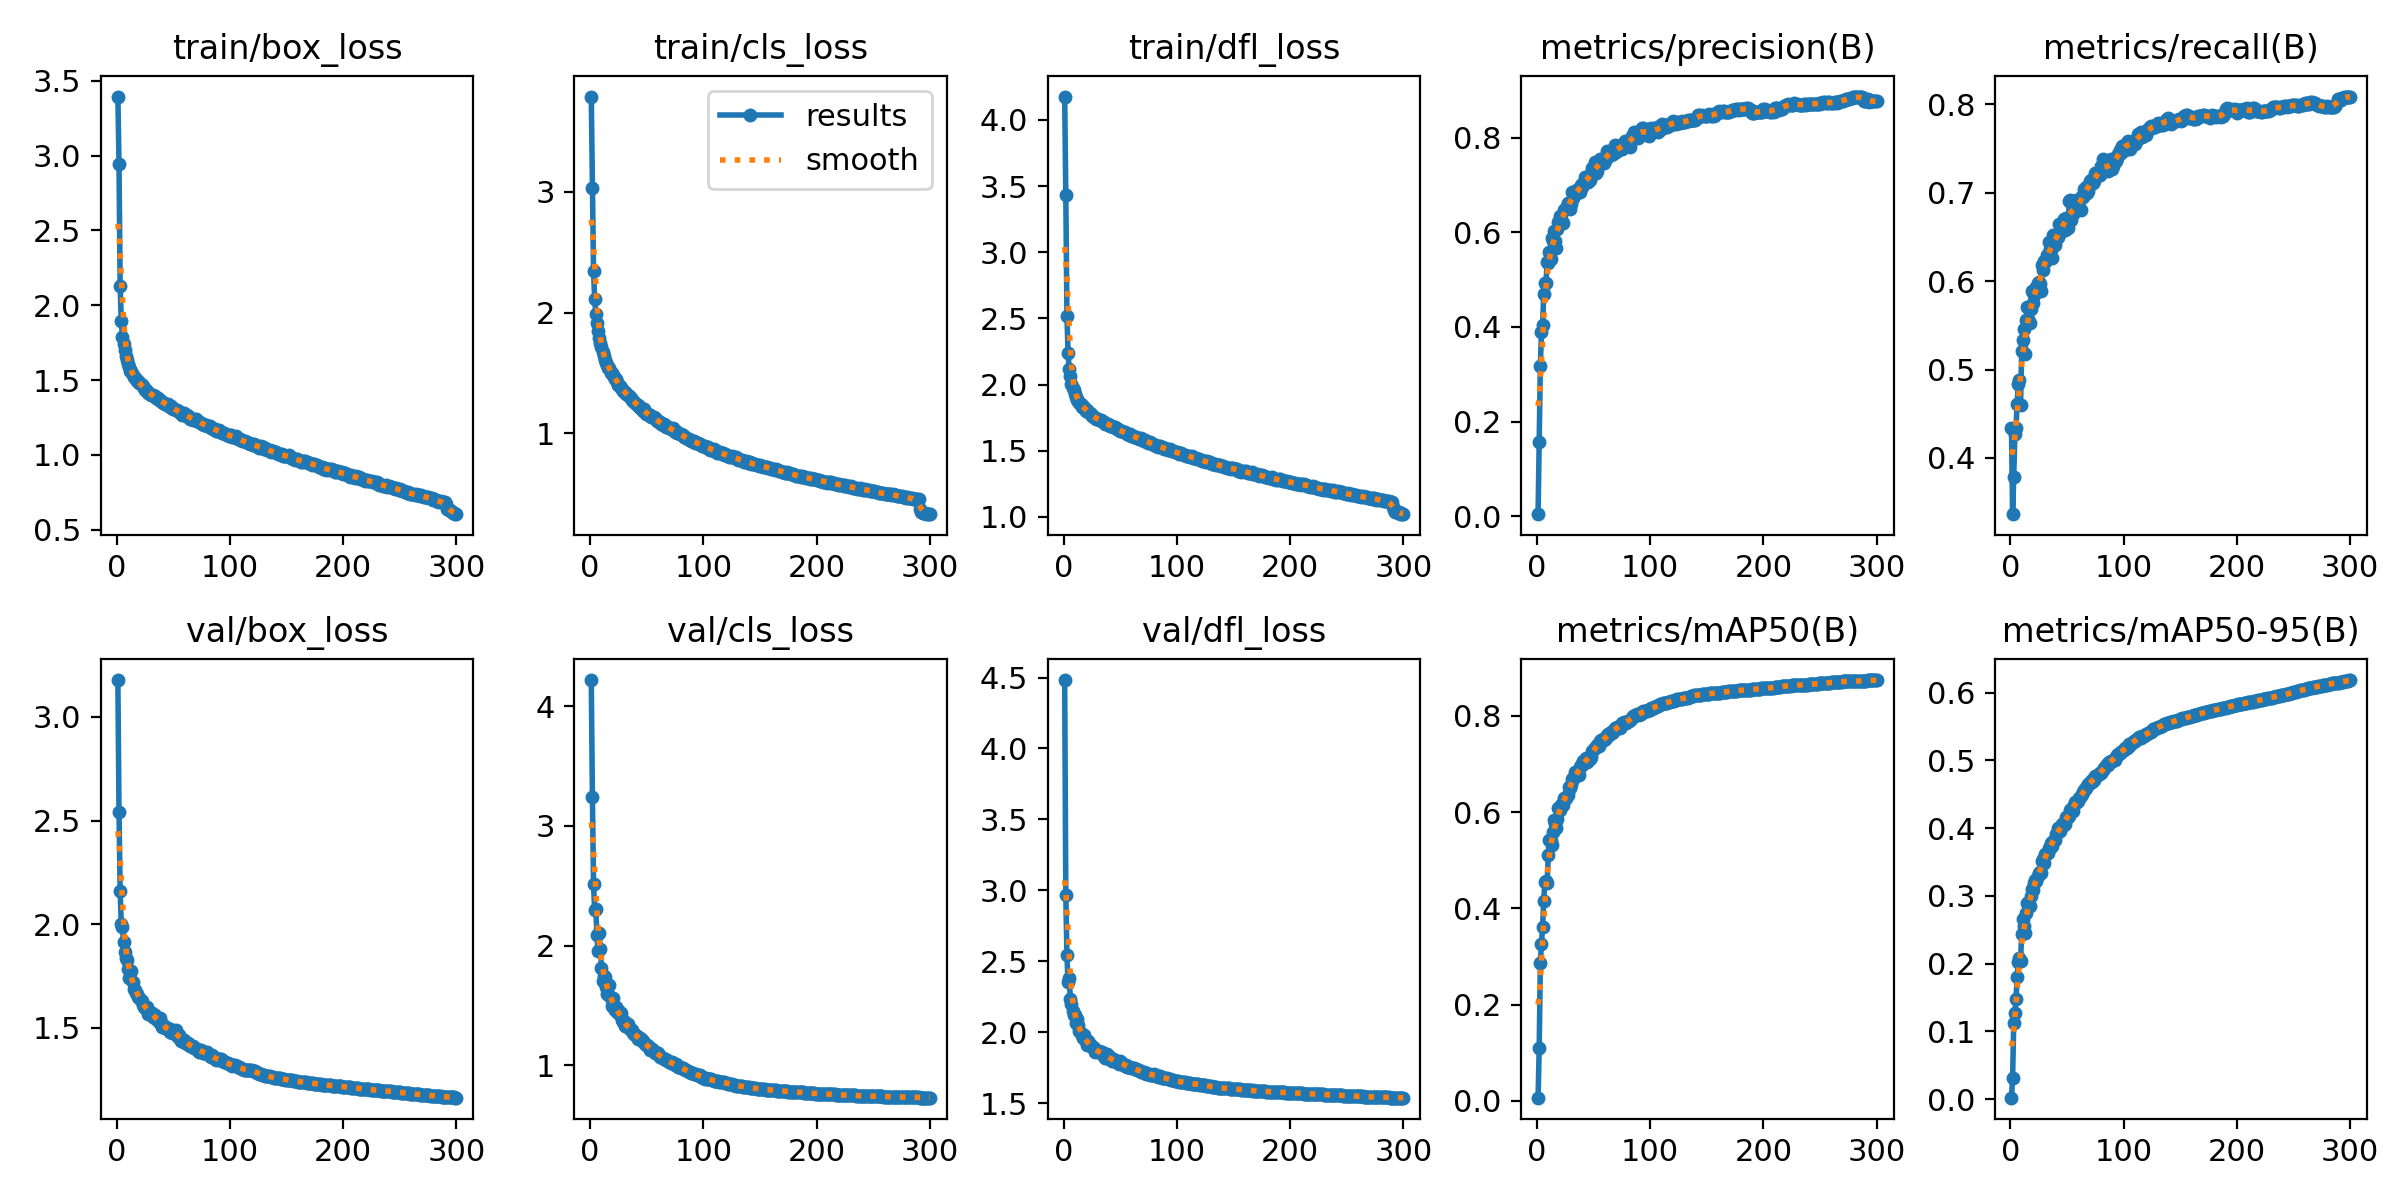
\includegraphics[width=.96\linewidth,height=.74\textheight,keepaspectratio]{assets/curves/results.png}
  \par\vspace{.04cm}
  {\small 300 个 epoch 的训练记录；曲线来自本次 batch 40、从零初始化的完整训练。}
  \paperref{本次 300 epoch 训练曲线，服务器 results.png}
\end{frame}

\begin{frame}{验证集诊断：漏检与背景误报都要看}
  \begin{columns}[T,onlytextwidth]
    \begin{column}{.66\textwidth}
      \centering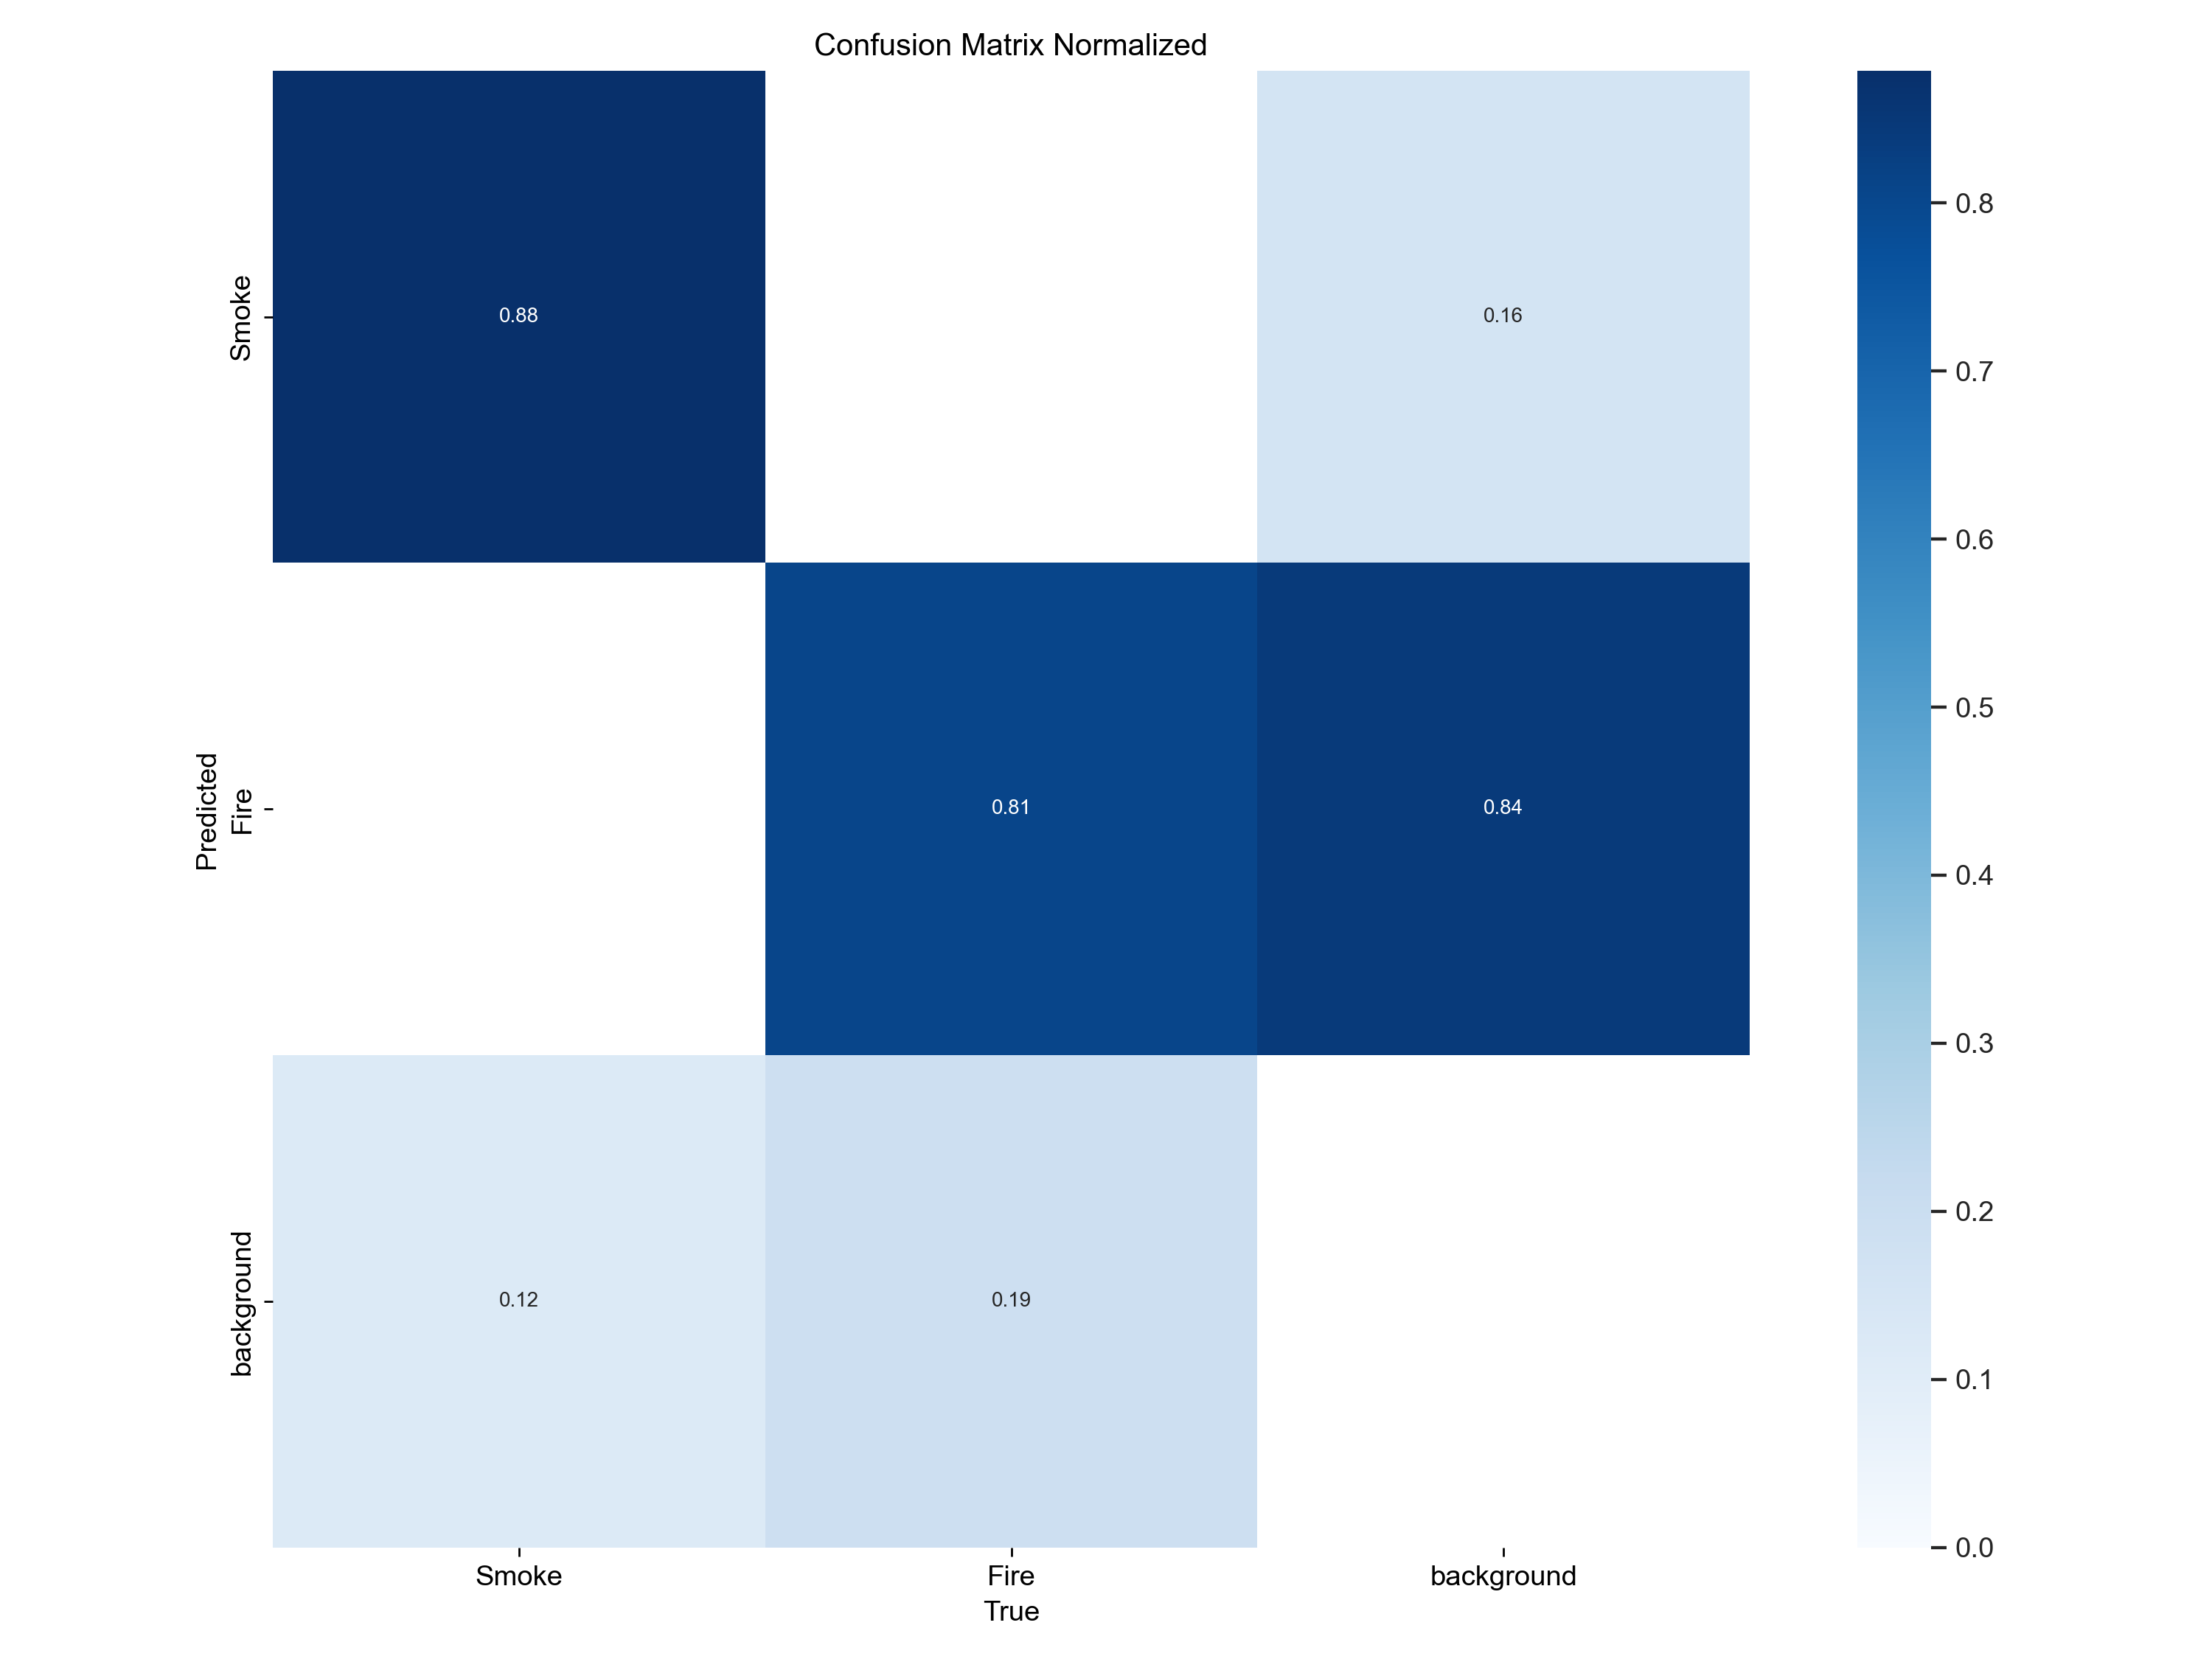
\includegraphics[width=\linewidth,height=.62\textheight,keepaspectratio]{assets/curves/confusion_matrix_normalized.png}
    \end{column}
    \begin{column}{.31\textwidth}
      \begin{itemize}
        \item Smoke 约 88\% 落在正确类别；Fire 约 81\%。
        \item 背景误报里，约 84\% 的未匹配预测属于 Fire 类。
        \item 背景误报会影响监控场景的实际告警负担。
      \end{itemize}
    \end{column}
  \end{columns}
  \vfill\scriptsize 这是训练过程中的验证集归一化混淆矩阵，不是独立测试集指标。
  \paperref{训练验证集；best.pt}
\end{frame}

\begin{frame}{独立测试集结果：Smoke 好于 Fire}
  \begin{columns}[T,onlytextwidth]
    \begin{column}{.55\textwidth}
      \renewcommand{\arraystretch}{1.42}
      \begin{tabular}{lrrrr}
        \toprule
        类别 & Precision & Recall & AP@0.5 & AP@0.5:0.95\\
        \midrule
        Smoke & 0.899 & 0.838 & 0.894 & 0.684\\
        Fire & 0.835 & 0.746 & 0.830 & 0.531\\
        \midrule
        总体 & 0.867 & 0.792 & 0.862 & 0.608\\
        \bottomrule
      \end{tabular}
      \vspace{.25cm}
      \small 测试集：1,059 张图、3,162 个标注框。
    \end{column}
    \begin{column}{.40\textwidth}
      \Large\bfseries 结论怎么读\par\medskip
      \normalsize
      \begin{itemize}
        \item mAP@0.5 = 86.2\%：在较宽松的框重合标准下，整体检测较好。
        \item mAP@0.5:0.95 = 60.8\%：严格定位标准下还有改进空间。
        \item Smoke AP 高于 Fire 6.4 个百分点；小火和复杂背景值得继续查错。
      \end{itemize}
    \end{column}
  \end{columns}
  \paperref{best.pt 在固定 test split 上验证}
\end{frame}

\begin{frame}{测试图像上的实际预测}
  \begin{columns}[T,onlytextwidth]
    \begin{column}{.32\textwidth}
      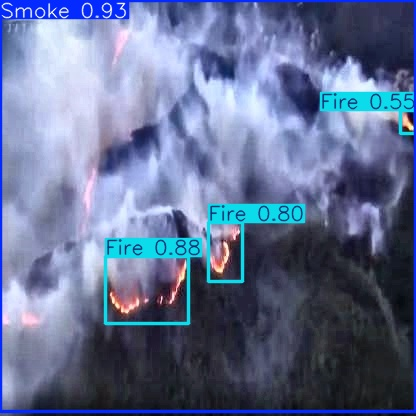
\includegraphics[width=\linewidth,height=.46\textheight,keepaspectratio]{assets/predictions/test_smoke_fire.jpg}
      \par\centering{\scriptsize 烟雾 + 火焰}
    \end{column}
    \begin{column}{.32\textwidth}
      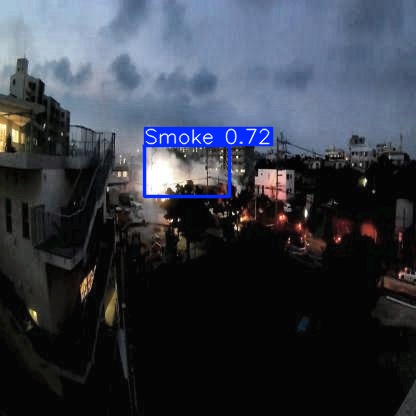
\includegraphics[width=\linewidth,height=.46\textheight,keepaspectratio]{assets/predictions/test_smoke.jpg}
      \par\centering{\scriptsize 烟雾}
    \end{column}
    \begin{column}{.32\textwidth}
      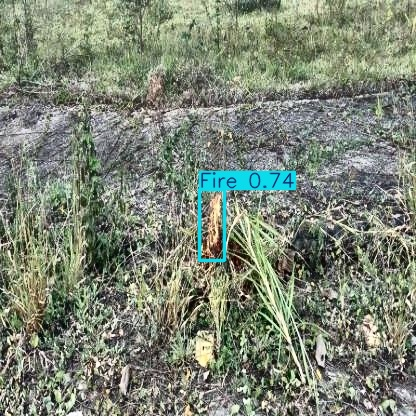
\includegraphics[width=\linewidth,height=.46\textheight,keepaspectratio]{assets/predictions/test_fire.jpg}
      \par\centering{\scriptsize 火焰}
    \end{column}
  \end{columns}
  \vspace{.15cm}
  \small best.pt 在独立测试图像上给出火与烟的框和置信度；总体效果以整套测试指标为准。
  \paperref{固定 test split 样例；置信度阈值 0.25}
\end{frame}

\begin{frame}{复现图像 1/8：烟雾框定位较准}
  \centering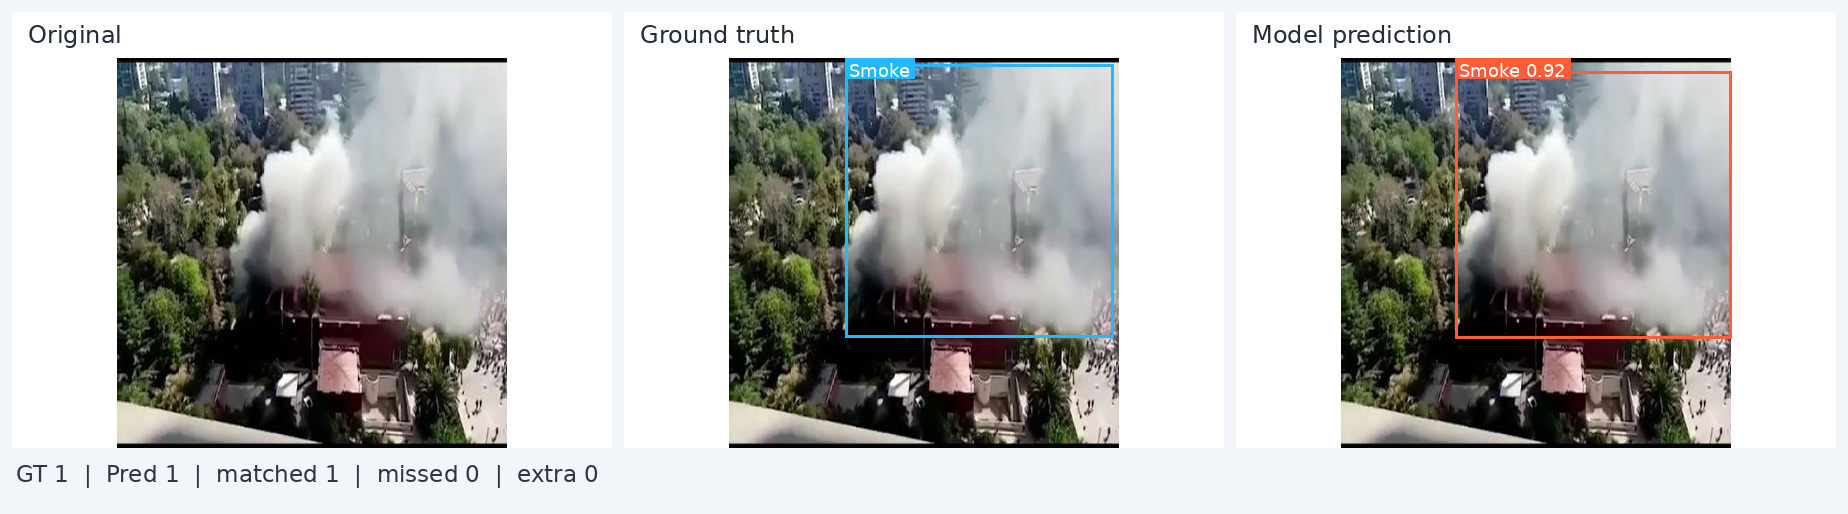
\includegraphics[width=.98\linewidth,height=.63\textheight,keepaspectratio]{assets/comparisons/case_01_smoke.jpg}
  \par\small 烟雾：标注 1 框、预测 1 框；IoU 0.949，置信度 0.921。
  \paperref{蓝/紫框为标注，红框为预测；输入为 CLAHE+CS 图；固定测试集样例}
\end{frame}

\begin{frame}{复现图像 2/8：烟雾边缘带来框位置偏差}
  \centering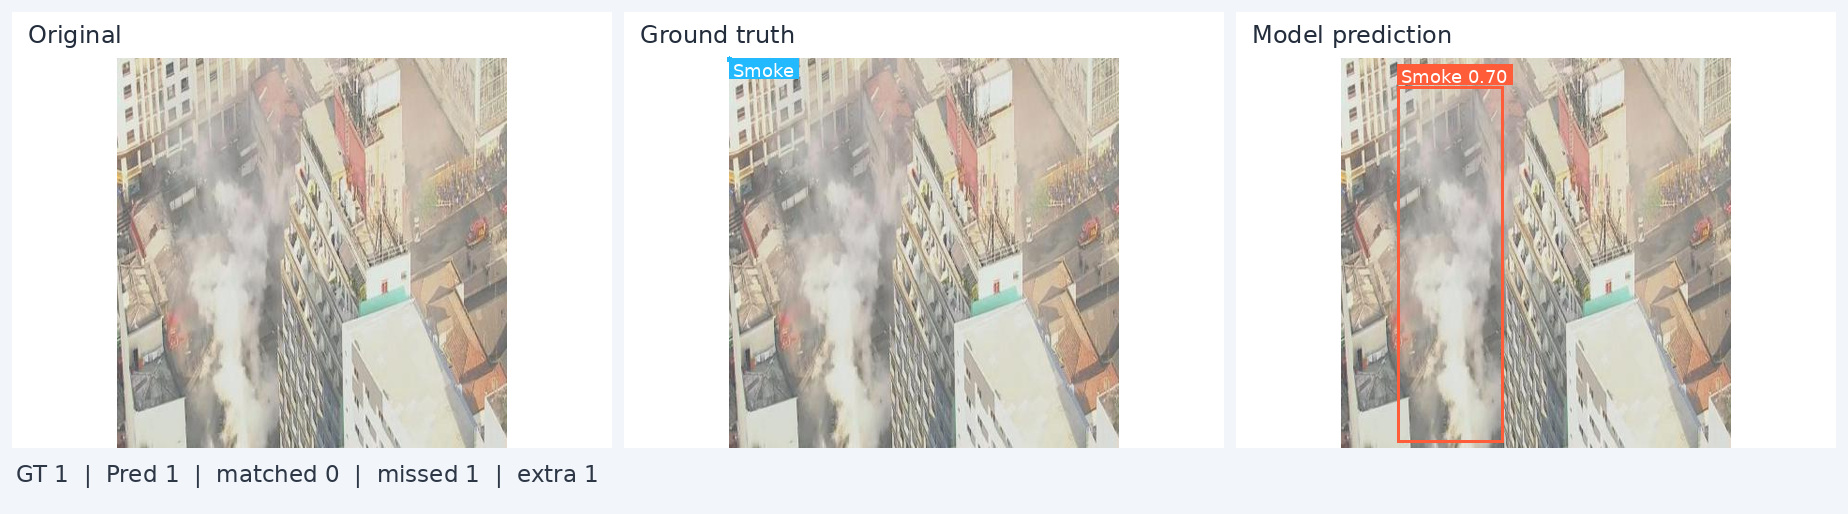
\includegraphics[width=.98\linewidth,height=.63\textheight,keepaspectratio]{assets/comparisons/case_02_smoke.jpg}
  \par\small 标注与预测各 1 框，但同类别框的 IoU 未达到 0.5。
  \paperref{模型输入为 CLAHE+CS 图；预测框叠加在原图；固定测试集样例}
\end{frame}

\begin{frame}{复现图像 3/8：烟雾检测与标注接近}
  \centering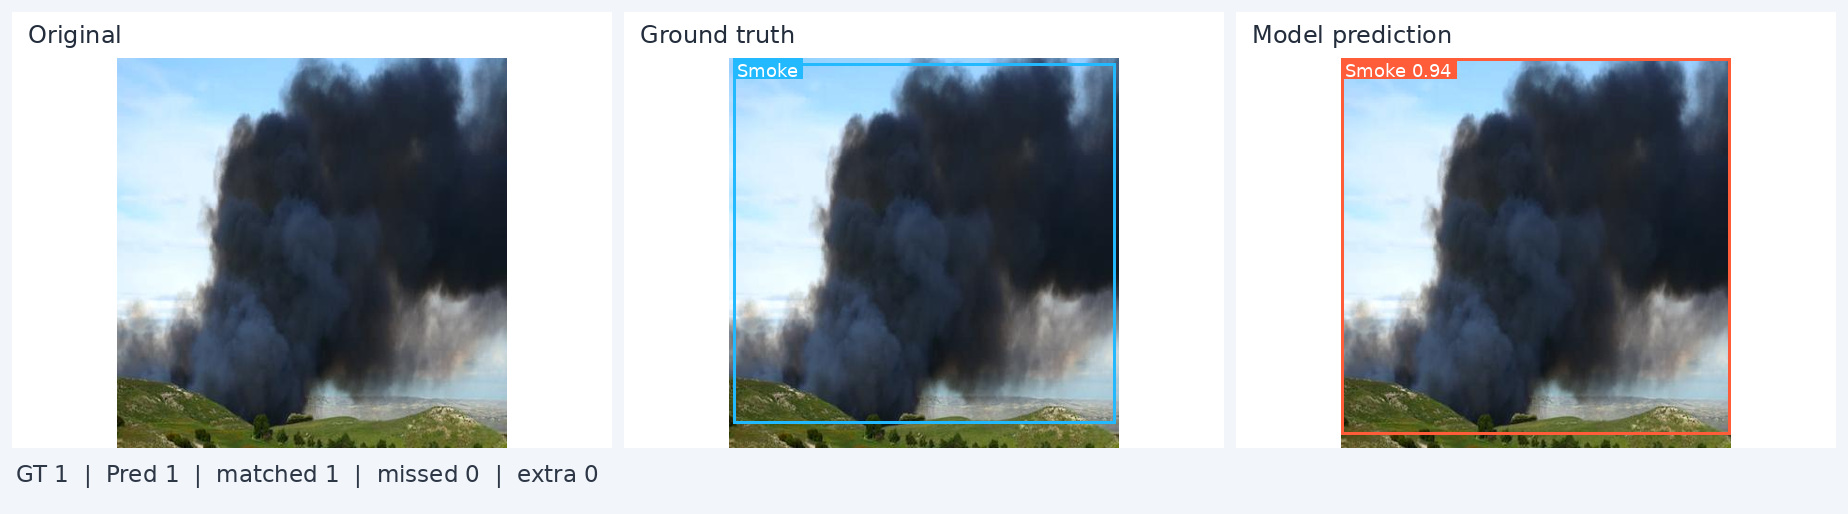
\includegraphics[width=.98\linewidth,height=.63\textheight,keepaspectratio]{assets/comparisons/case_03_smoke.jpg}
  \par\small 烟雾：标注 1 框、预测 1 框；IoU 0.936，置信度 0.944。
  \paperref{蓝/紫框为标注，红框为预测；固定测试集样例}
\end{frame}

\begin{frame}{复现图像 4/8：单个火焰定位较准}
  \centering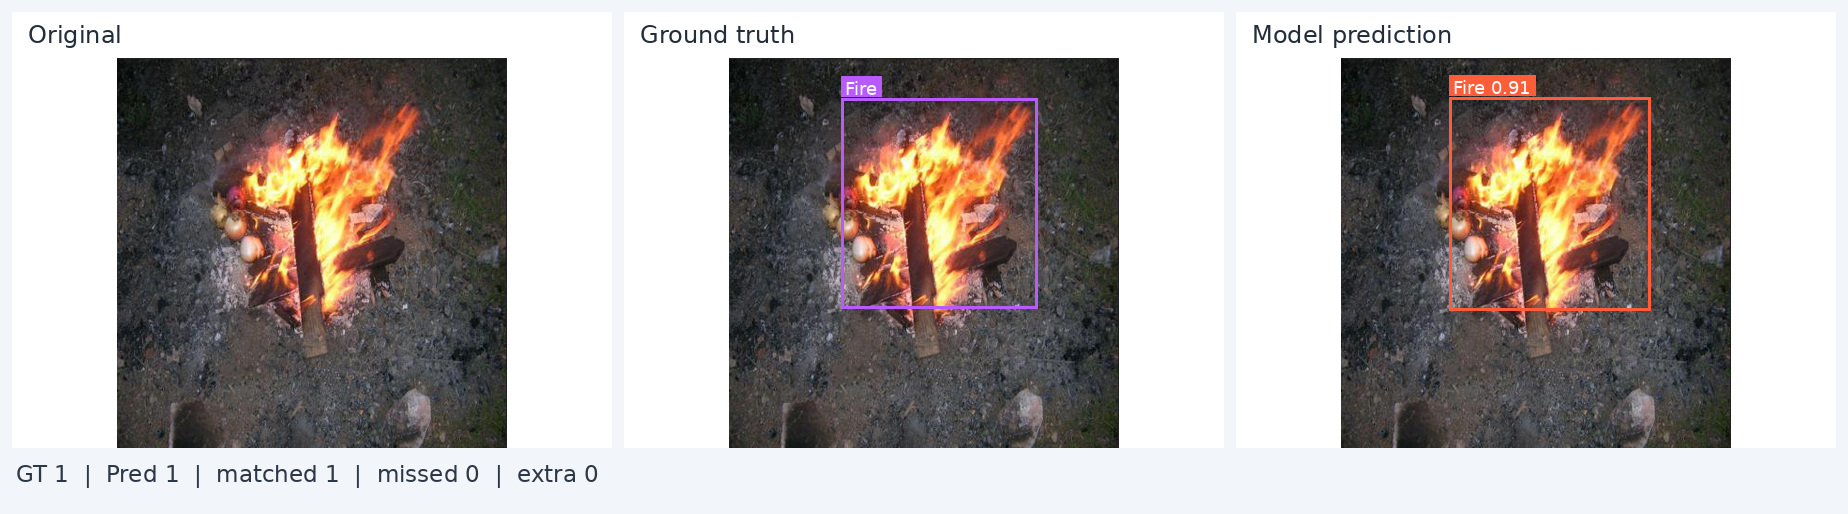
\includegraphics[width=.98\linewidth,height=.63\textheight,keepaspectratio]{assets/comparisons/case_04_fire.jpg}
  \par\small 火焰：标注 1 框、预测 1 框；IoU 0.961，置信度 0.911。
  \paperref{蓝/紫框为标注，红框为预测；固定测试集样例}
\end{frame}

\begin{frame}{复现图像 5/8：相邻火焰容易被合并}
  \centering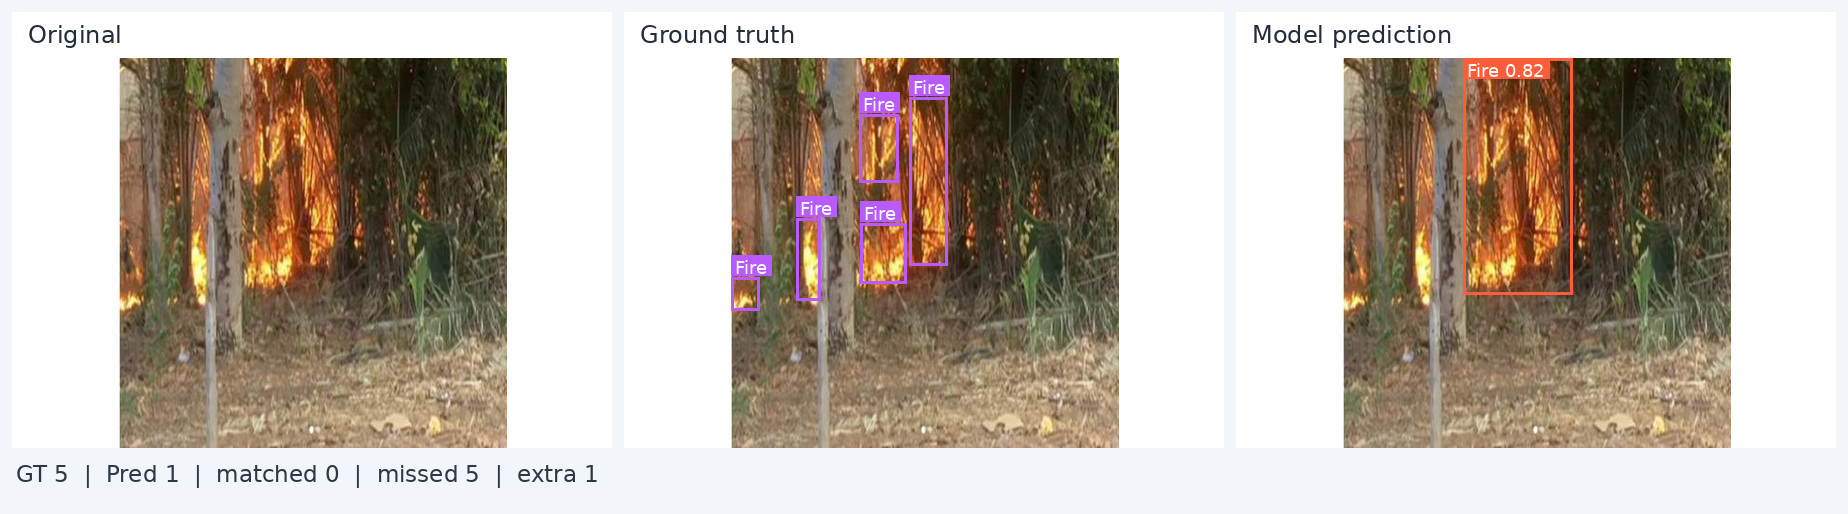
\includegraphics[width=.98\linewidth,height=.63\textheight,keepaspectratio]{assets/comparisons/case_05_fire.jpg}
  \par\small 标注 5 个火焰框，模型输出 1 个较大的框；按 IoU 0.5 标准均未匹配。
  \paperref{模型能指出火焰区域，但框的拆分和定位仍有误差；固定测试集样例}
\end{frame}

\begin{frame}{复现图像 6/8：单个火焰框匹配}
  \centering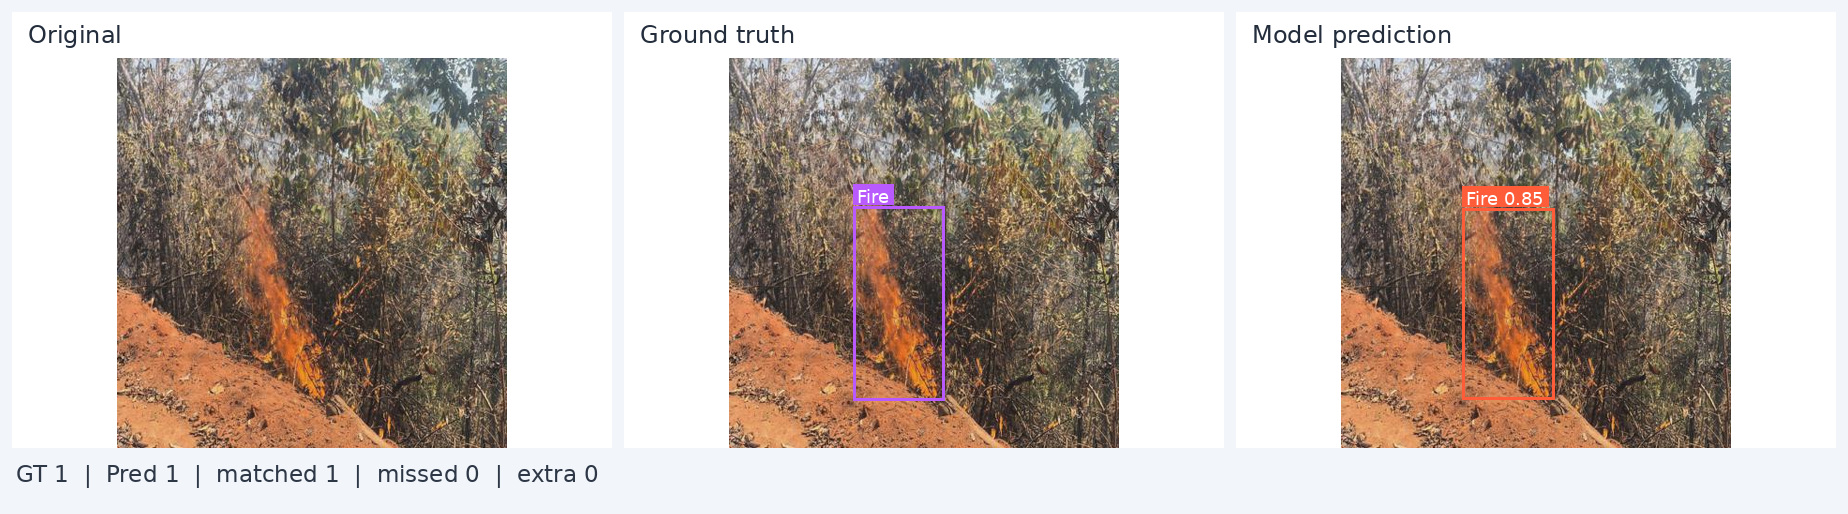
\includegraphics[width=.98\linewidth,height=.63\textheight,keepaspectratio]{assets/comparisons/case_06_fire.jpg}
  \par\small 火焰：标注 1 框、预测 1 框；IoU 0.943，置信度 0.848。
  \paperref{蓝/紫框为标注，红框为预测；固定测试集样例}
\end{frame}

\begin{frame}{复现图像 7/8：火焰与烟雾同时检出}
  \centering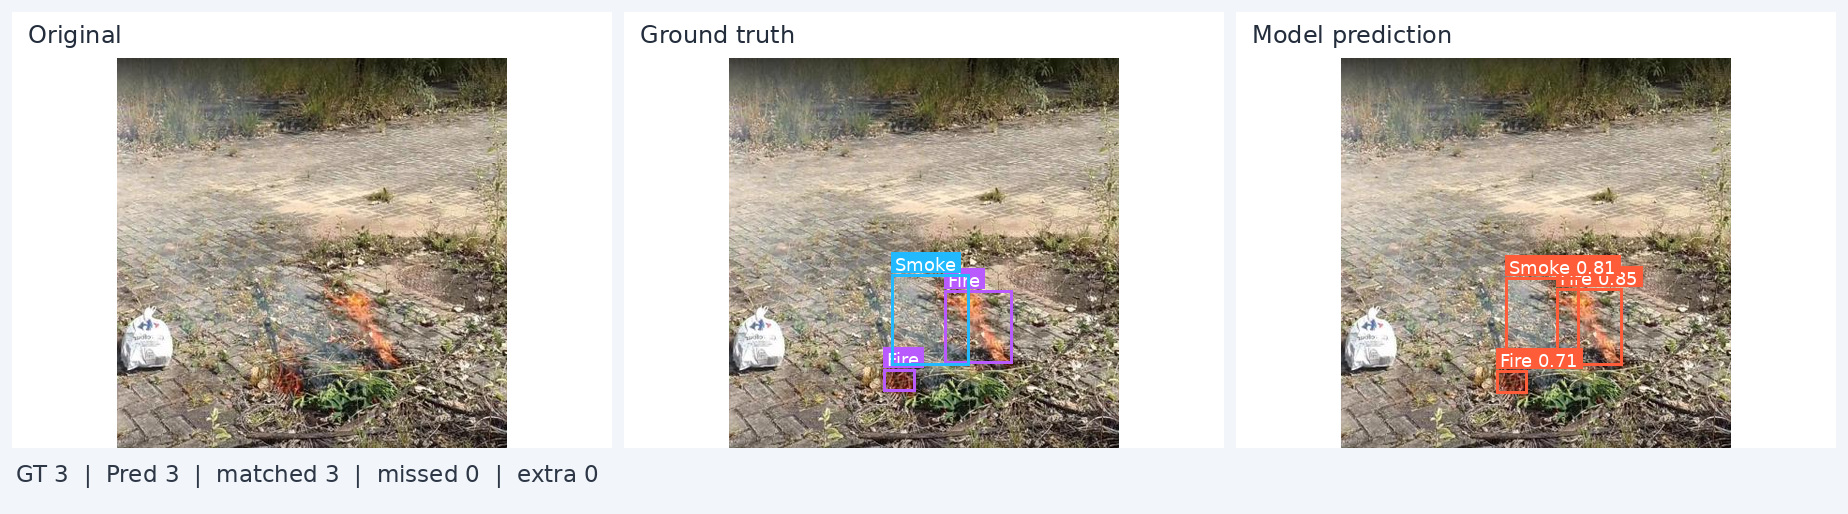
\includegraphics[width=.98\linewidth,height=.63\textheight,keepaspectratio]{assets/comparisons/case_07_mixed.jpg}
  \par\small 火烟同框：3 个标注框与 3 个预测框均满足同类别、IoU $\geq 0.5$。
  \paperref{蓝/紫框为标注，红框为预测；固定测试集样例}
\end{frame}

\begin{frame}{复现图像 8/8：火烟混杂的困难样例}
  \centering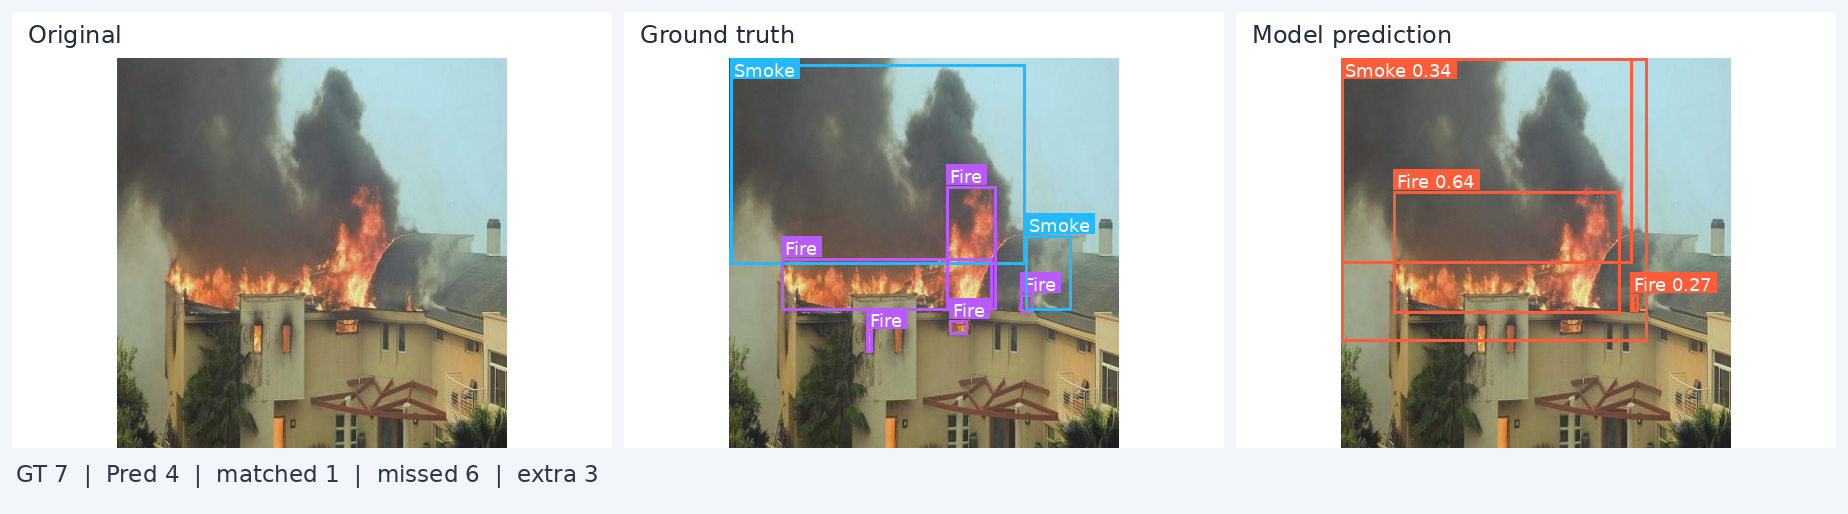
\includegraphics[width=.98\linewidth,height=.63\textheight,keepaspectratio]{assets/comparisons/case_08_mixed.jpg}
  \par\small 标注 7 框、预测 4 框；同类别且 IoU $\geq 0.5$ 的匹配 1 框，另有 6 个标注框未匹配。
  \paperref{这些是定性例图，不代表测试集平均表现；存在框位置与标注差异}
\end{frame}

\begin{frame}{所以，这次训练有效果吗？}
  \begin{columns}[T,onlytextwidth]
    \begin{column}{.49\textwidth}
      \begin{block}{可以确认的}
        \begin{itemize}
          \item 完成 300 轮训练，loss 收敛。
          \item 独立测试集总体 mAP@0.5 为 86.2\%。
          \item 火焰、烟雾都能检出，测试图上可看到对应框。
        \end{itemize}
        \textbf{结论：}有实际检测效果，可作为后续实验的起点。
      \end{block}
    \end{column}
    \begin{column}{.47\textwidth}
      \begin{alertblock}{还不能下的结论}
        \begin{itemize}
          \item 论文摘要报告 89.50\% mAP；公开页面未在该数值旁标明与本次相同的 mAP 阈值。
          \item 本次从零初始化，代码结构和增强细节也有实现选择。
          \item 单次训练、单一数据集，不能证明复杂野外场景都可靠。
        \end{itemize}
      \end{alertblock}
    \end{column}
  \end{columns}
  \vspace{.15cm}
  \centering\small\textbf{有检测效果；但不能据此说已严格复现论文或达到部署要求}
  \paperref{论文报告值见 ScienceDirect Highlights；本次指标见固定测试集评估}
\end{frame}

\begin{frame}{局限与可以继续做的方向}
  \begin{columns}[T,onlytextwidth]
    \begin{column}{.48\textwidth}
      \textbf{当前局限}\par\medskip
      \begin{itemize}
        \item 烟雾边界模糊，框的精确位置仍不稳定。
        \item 当前只在一个公开数据集上评估，没按云雾、逆光、夜间拆分误报率。
        \item 只有一次随机种子；尚未做逐模块消融。
      \end{itemize}
    \end{column}
    \begin{column}{.48\textwidth}
      \textbf{后续研究思路}\par\medskip
      \begin{enumerate}
        \item 用同一训练协议比较从零训练与预训练初始化。
        \item 加入视频连续帧信息，过滤短暂烟尘和光照误报。
        \item 对烟雾尝试分割或边界不确定性建模，不只回归矩形框。
        \item 跨数据集测试，按白天/夜间、云雾、逆光分别统计结果。
      \end{enumerate}
    \end{column}
  \end{columns}
  \vspace{.2cm}
  \begin{block}{可借鉴的核心思路}
    先定位真实困难，再分别从输入图像、特征提取和多尺度融合入手；用分场景评估验证每个改动是否真有帮助。
  \end{block}
  \paperref{基于论文方法与本次复现局限提出的后续方向}
\end{frame}

\begin{frame}{参考文献与复现资源}
  \small
  \begin{enumerate}
    \item C. Dewi, D. Thiruvady, S. A. Philemon, N. Zaidi. “Improving fire and smoke detection with ghost convolutions, Bidirectional Feature Pyramid Networks, and image enhancement.” \emph{Engineering Applications of Artificial Intelligence}, 178 (2026), 115116. DOI: \url{https://doi.org/10.1016/j.engappai.2026.115116}.
    \item 官方代码仓库：\url{https://github.com/ChristineDewi/YOLO_GN}
    \item Fire and Smoke Dataset：\url{https://github.com/vinchole/zzzccc}
    \item 期刊分区：科研通，Engineering Applications of Artificial Intelligence，2025 年中科院升级版分区页面。
    \item 复现记录、模型 YAML、训练脚本与测试结果：本项目 \texttt{README.md}、\texttt{复现进度.md}、\texttt{models/}、\texttt{scripts/}。
  \end{enumerate}
  \vspace{.35cm}
  \centering\Large 谢谢
\end{frame}

\end{document}
